\section{Mediciones}

Para las mediciones, creamos listas de compilados de ejemplo de forma aleatoria. Decidimos que el tiempo
de análisis de un compilado fuera un valor aleatorio entre 1 y 99'999, basándonos en los datos de ejemplo
provistos por la cátedra.

Medimos el tiempo de ejecución de nuestro algoritmo para ciertas cantidades de compilados. Notamos ciertas irregularidades en los tiempos de ejecución,
por lo que decidimos realizar varias mediciones para el mismo escenario de compilados y tomar el promedio de los tiempos obtenidos.
Además, como definimos cada escenario arbitrariamente, en una cantidad de compilados $x$, este escenario puede ser poco favorable (puede estar muy desordenado),
mientras que en una cantidad de compilados $x+1$ puede ser muy favorable. Por lo cual la diferencia de tiempos va a ser muy grande a pesar de que la cantidad
de compilados solamente difiere en una unidad (TimSort es una combinación de inserción y mergeSort, por lo cual el desorden inicial toma gran relevancia en el 
rendimiento final del algorítmo). Para evitar esto, decidimos hacer varios escenarios distintos para la misma cantidad de compilados, promediando a su vez, los 
tiempos de ejecución.

Con el objetivo de comparar los tiempos de ejecución de nuestro algoritmo con la complejidad teórica, optamos por 
realizar tanto un análisis de regresión lineal como uno de regresión lineal logarítmica que se ajustara a nuestros datos.
Ahora, debemos comprobar cuál de las dos curvas se ajusta mejor. Para ello, usamos la raíz del
error cuadrático medio, que nos da una idea de cuán cerca están los valores predichos de los valores reales.

\begin{figure}[H]
    \centering
    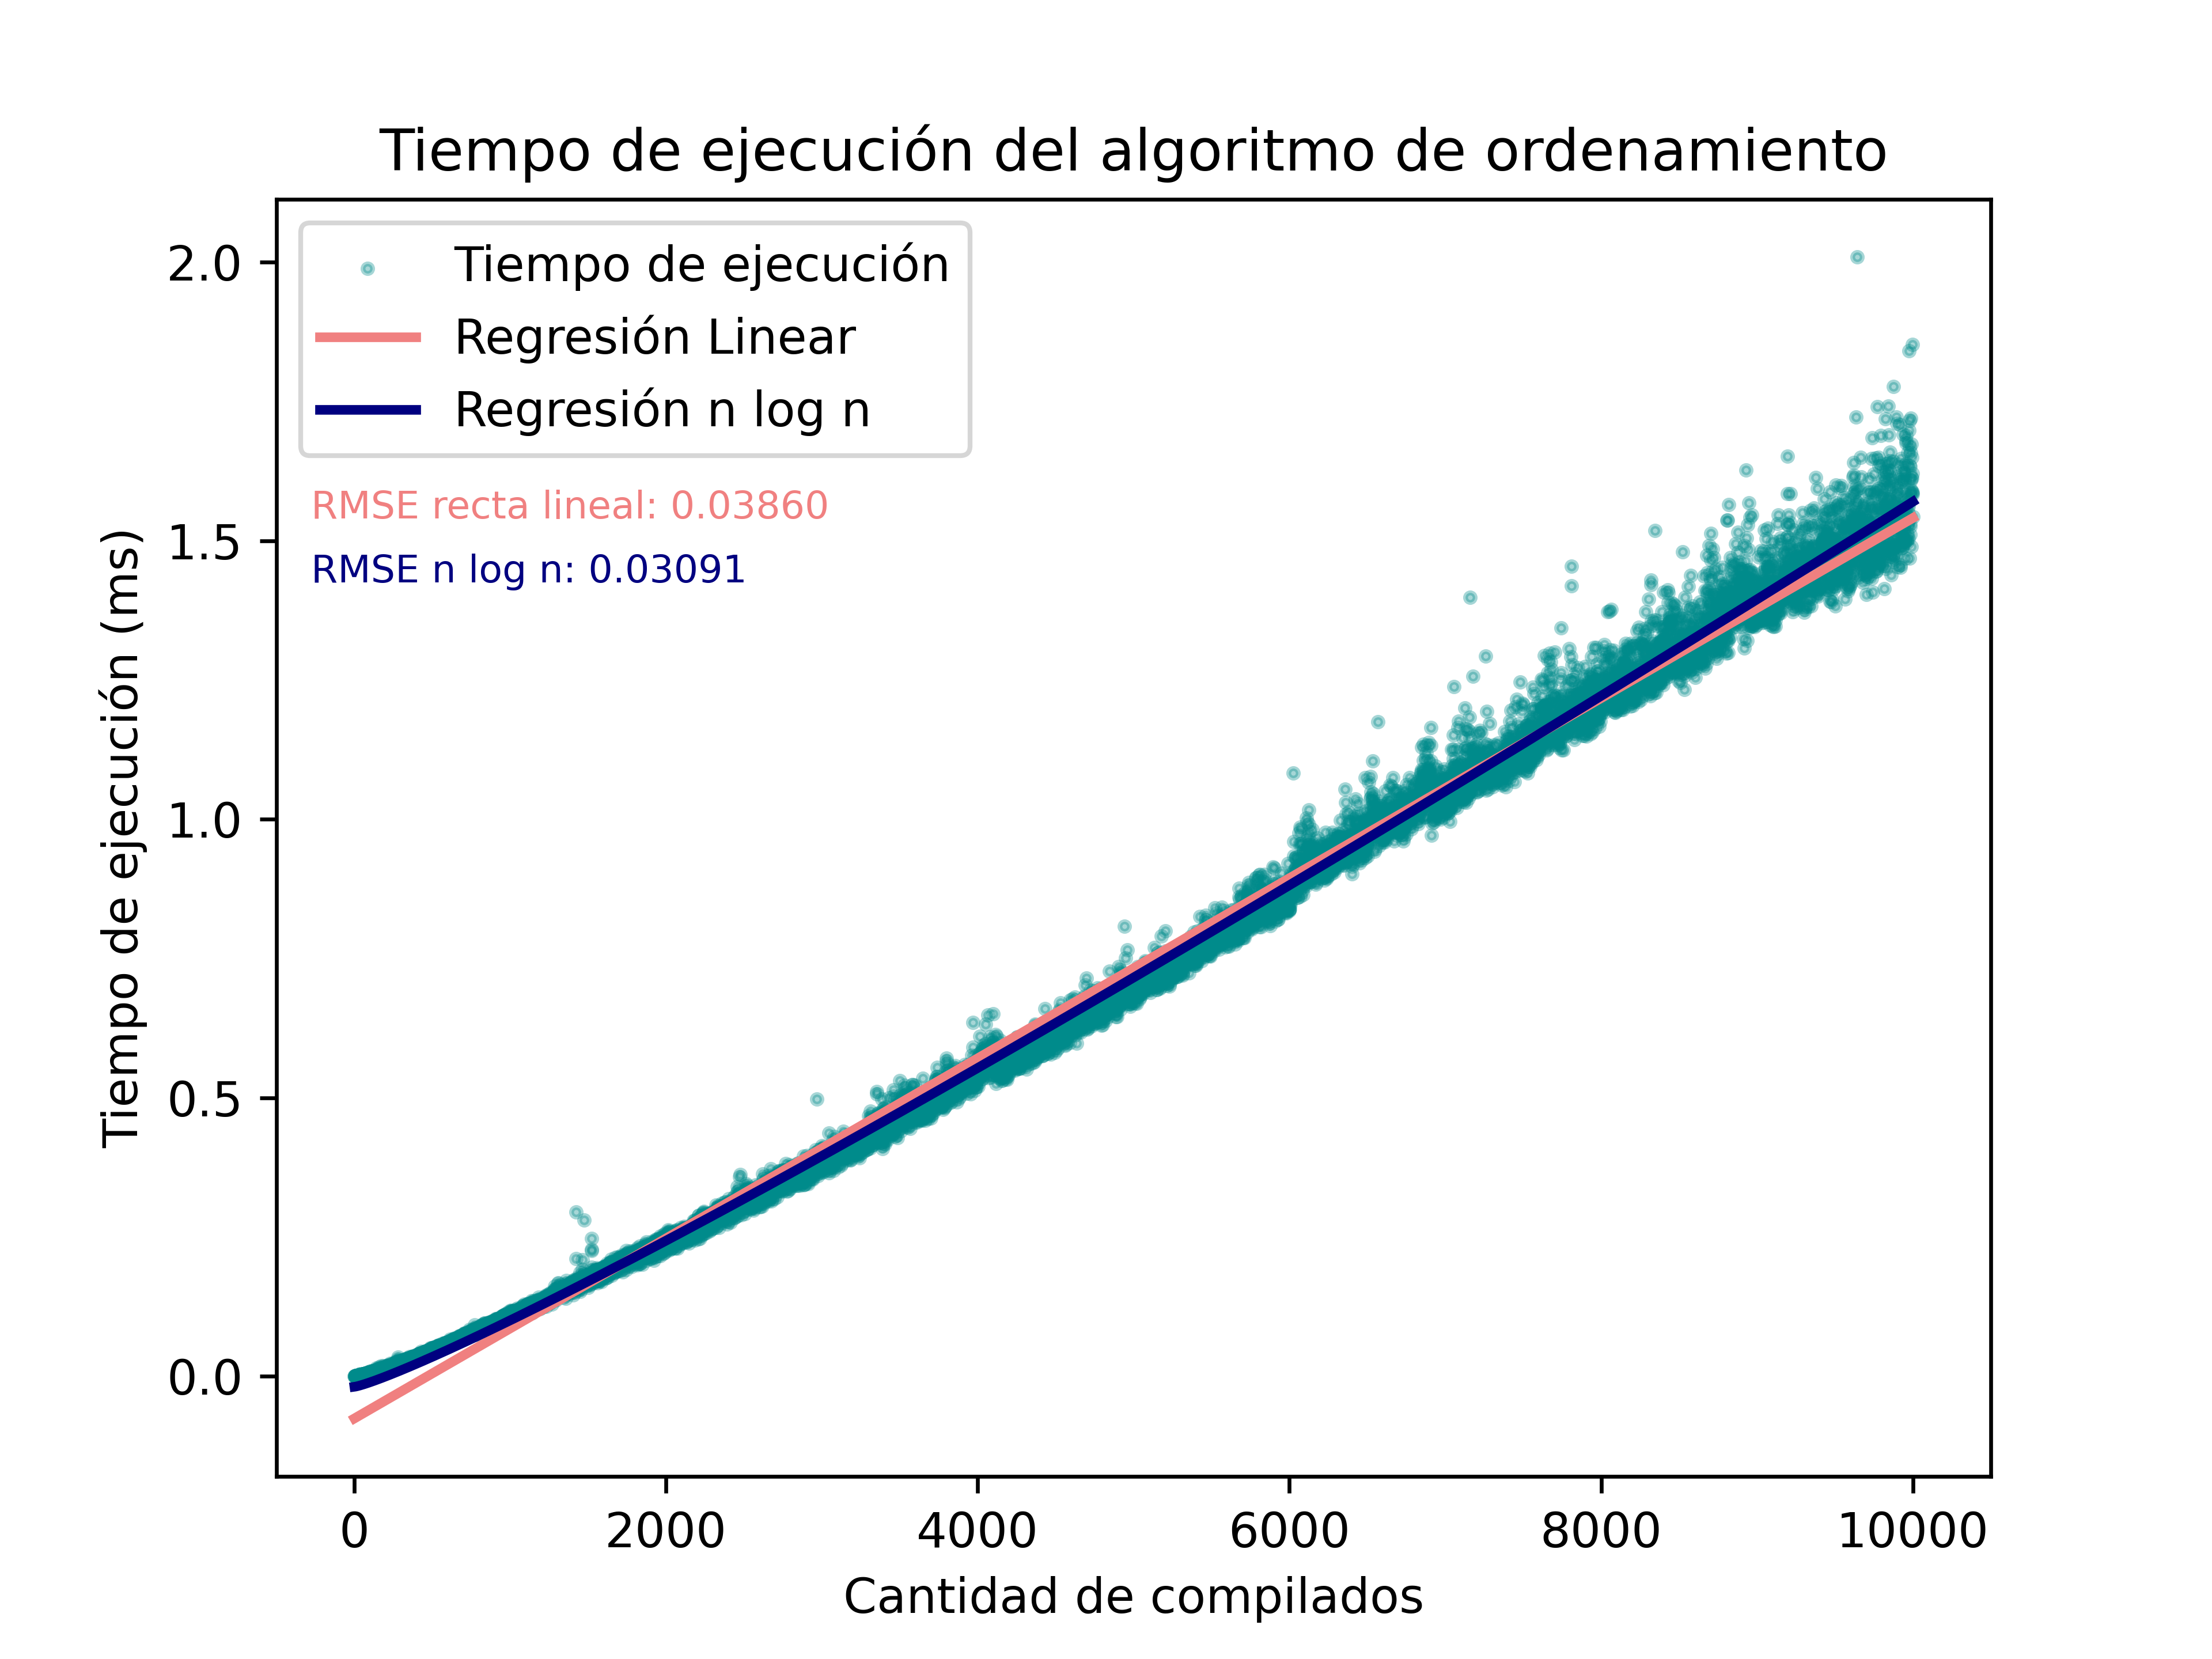
\includegraphics[width=1\textwidth]{img/tiempos_ejecucion.png}
\end{figure}

Al calcular el error cuadrático medio para ambas curvas, observamos que el error era prácticamente similar.
En consecuencia, decidimos llevar a cabo un análisis más detallado,
enfocándonos en diversos intervalos del gráfico con el objetivo de examinar el comportamiento de los datos en mayor
profundidad. Esta investigación nos permitió concluir que, especialmente en el caso de muestras caracterizadas
por valores reducidos, la curva lineal logarítmica se ajusta mejor a los datos observados.

% imagen de los tiempos de ejecucion zoom
\begin{figure}[H]
    \centering
    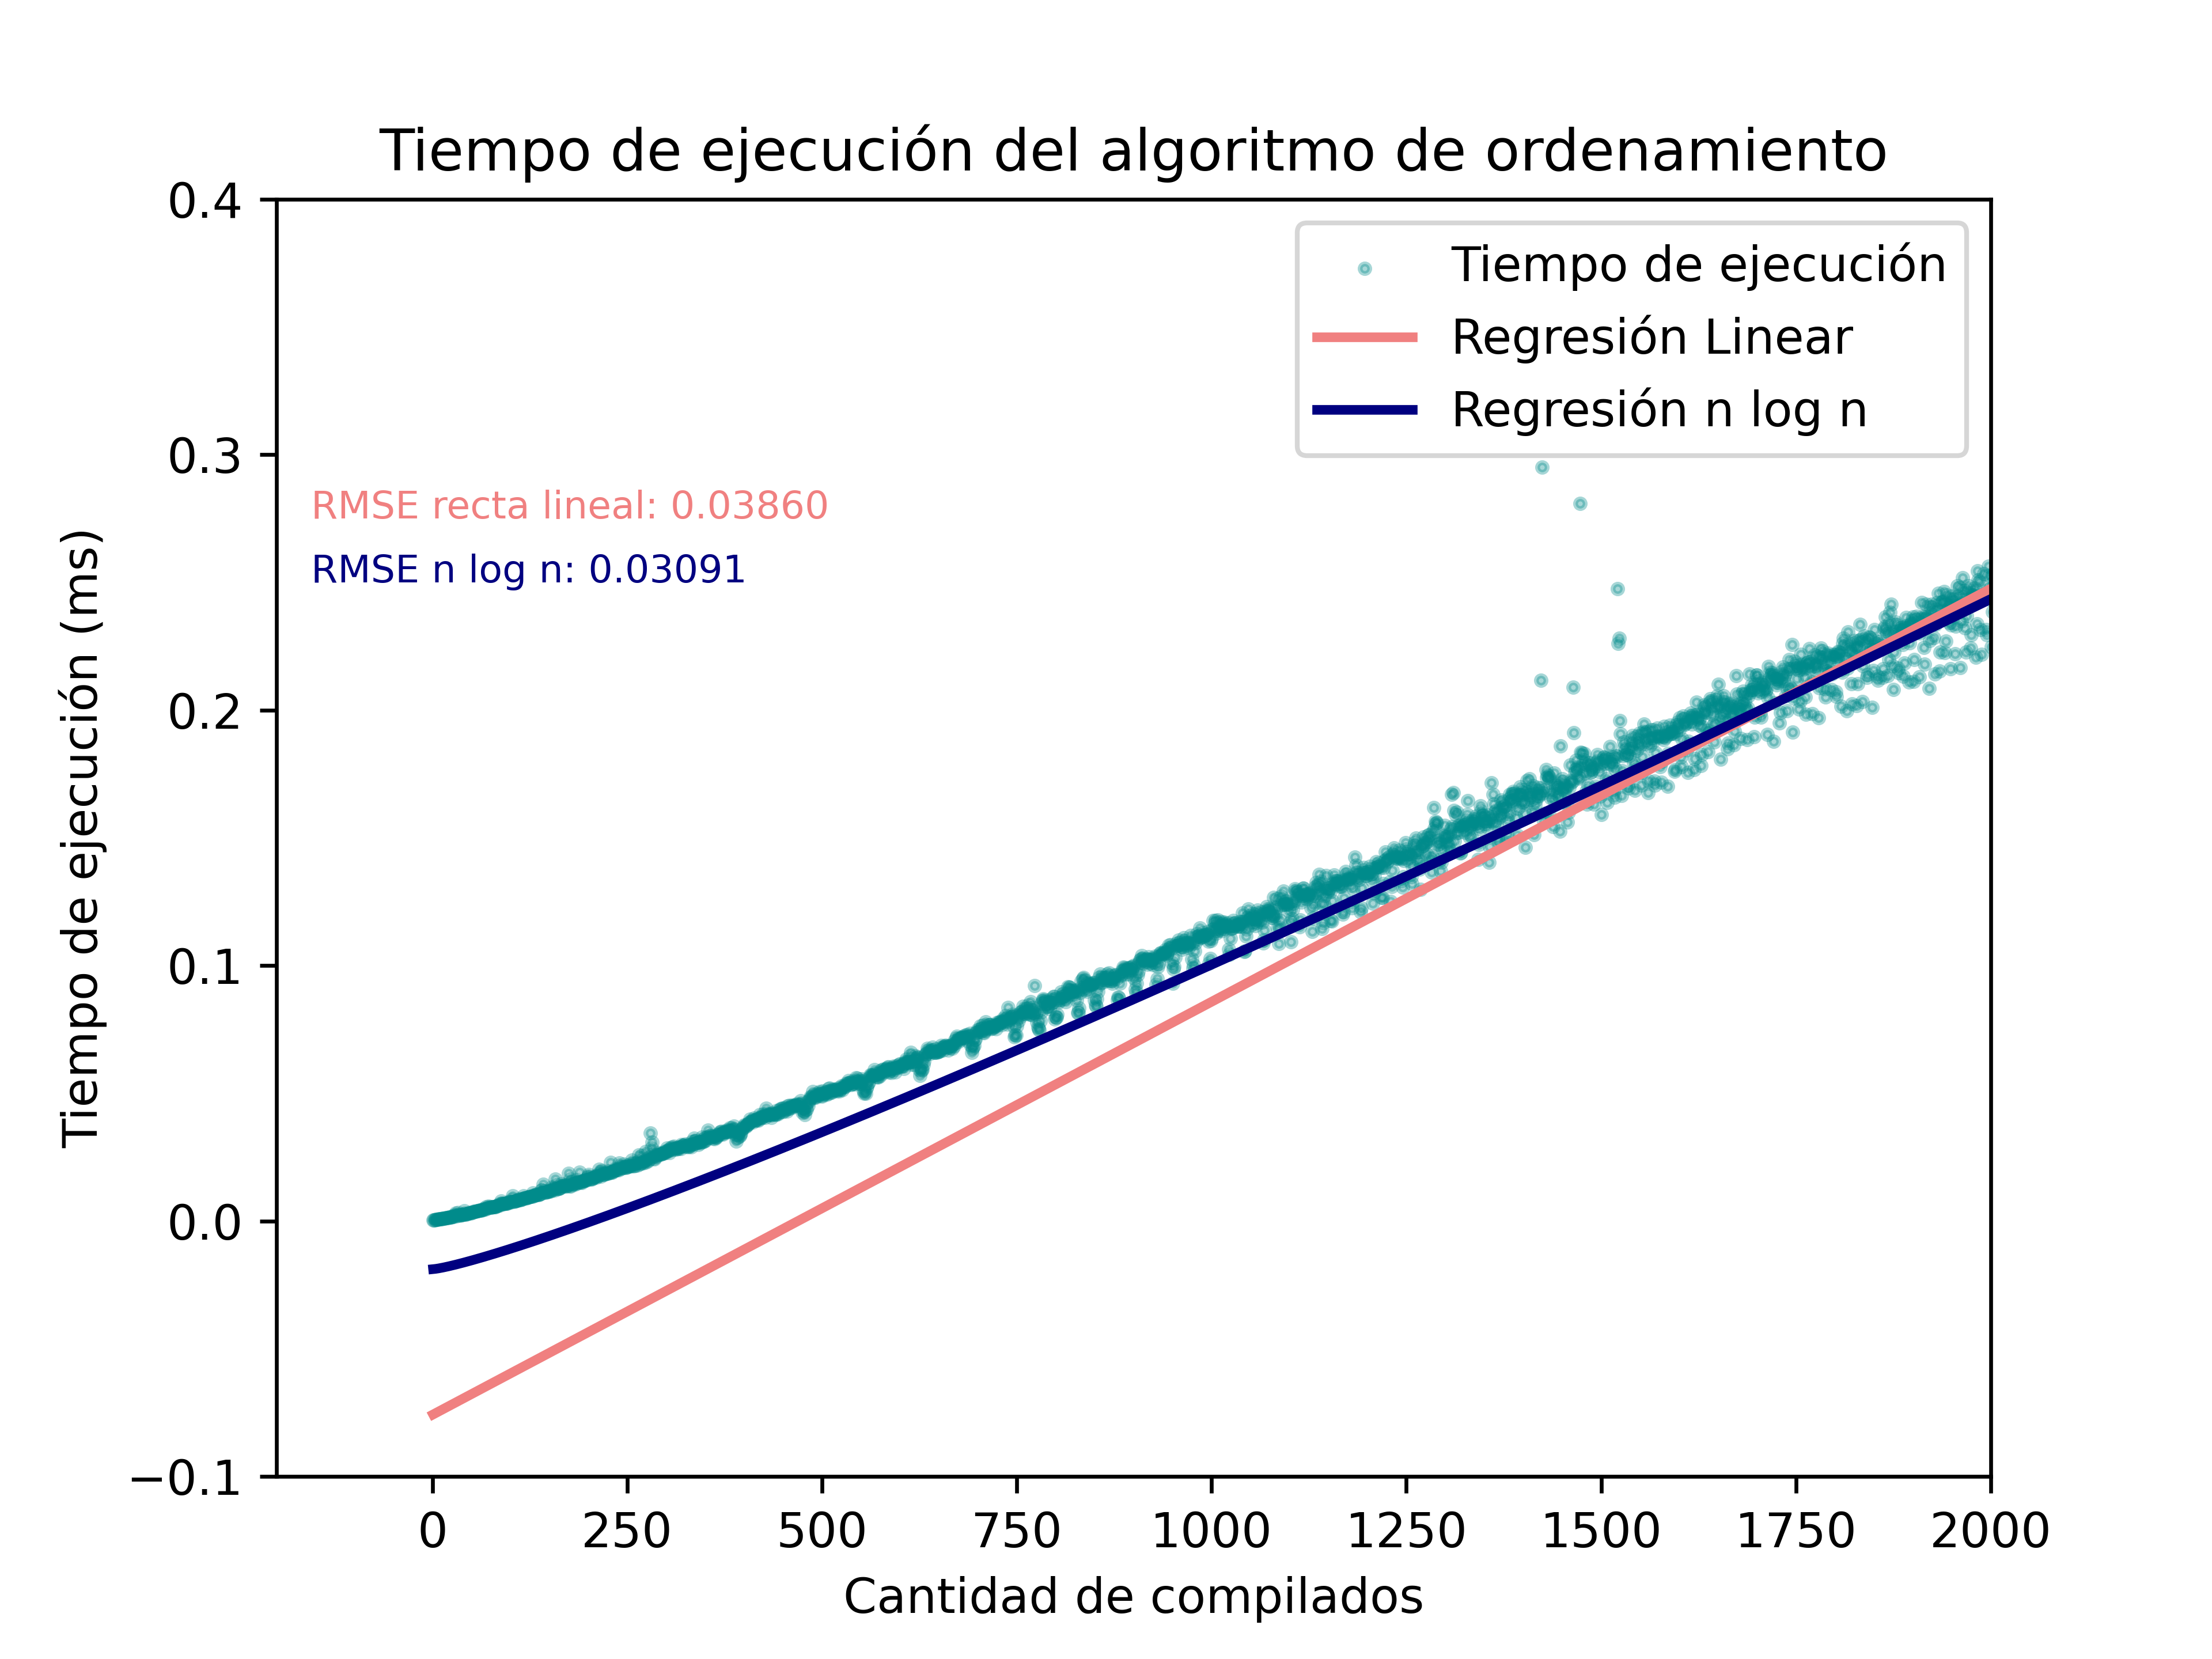
\includegraphics[width=1\textwidth]{img/tiempos_ejecucion_zoom_bajos.png}
\end{figure}

Sin embargo, al considerar valores más elevados, se observó que las diferencias en los tiempos tendieron a adquirir una naturaleza lineal.

% imagen de los tiempos de ejecucion zoom altos
\begin{figure}[H]
    \centering
    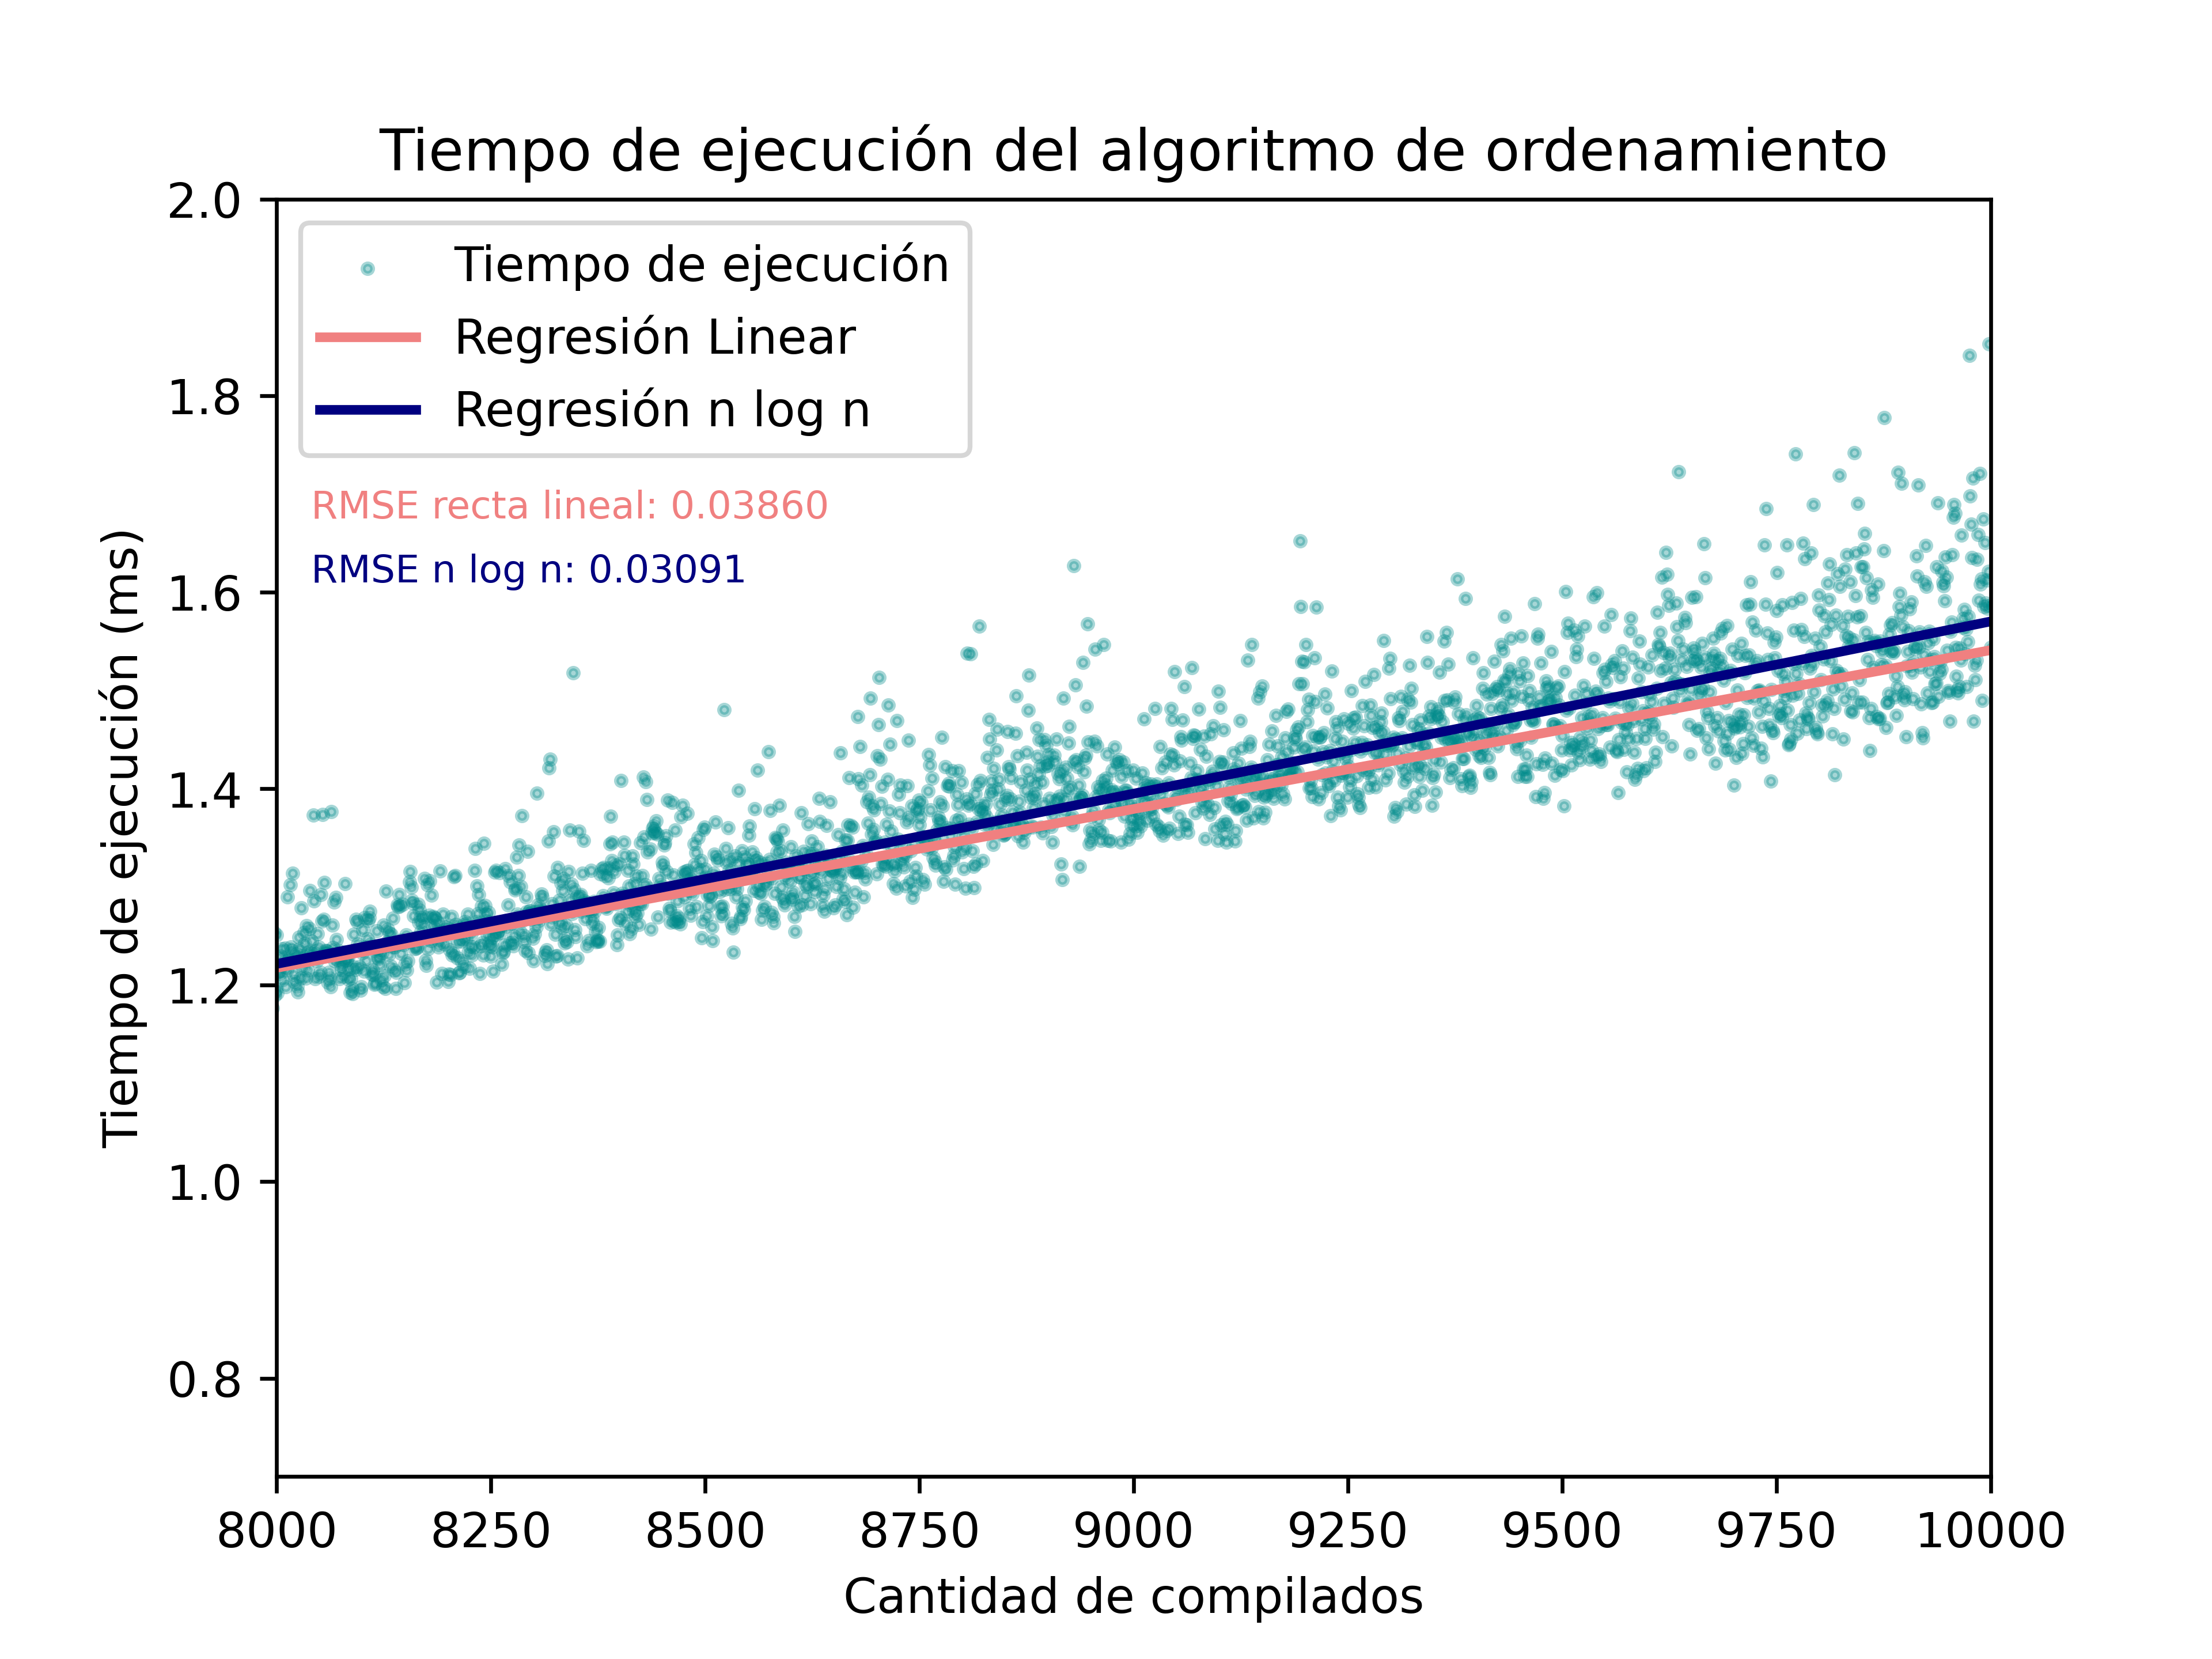
\includegraphics[width=1\textwidth]{img/tiempos_ejecucion_zoom_altos.png}
\end{figure}

Esto ocurre debido a la naturaleza de la función lineal logarítmica, que presenta una pendiente logarítmica. Cuando se 
trabajan con valores grandes, esta pendiente se vuelve casi constante, lo que la asemeja a una función lineal. Esto se 
debe a que el logaritmo es una función monótona creciente, lo que significa que su derivada es siempre positiva para valores 
mayores que cero. Sin embargo, el crecimiento de esta función se vuelve cada vez más lento a medida que los valores aumentan, 
indicando que su segunda derivada es siempre negativa. En consecuencia, para valores muy grandes, la función lineal logarítmica 
se estabiliza y, aunque no es completamente constante, su comportamiento se asemeja a una función lineal.

De esta manera, mediante el gráfico y la validación a través del error cuadrático medio, hemos comprobado que la curva lineal logarítmica 
se adapta de manera más precisa a nuestros datos.

De esta forma pudimos comprobar empíricamente que la complejidad tiende a $\operatorname{O}(n\log{n})$.